\documentclass[10pt,twocolumn]{article}
\usepackage[a4paper,margin=0.55in,columnsep=0.22in]{geometry}
\usepackage{amsmath,amssymb,graphicx,booktabs,hyperref,microtype}
\usepackage[font=small,skip=3pt]{caption}
\usepackage{titlesec}
\titlespacing*{\section}{0pt}{5pt}{2pt}
\titleformat*{\section}{\normalsize\bfseries}
\setlength{\parskip}{1pt}
\setlength{\abovedisplayskip}{3pt}\setlength{\belowdisplayskip}{3pt}
\hypersetup{colorlinks=true,urlcolor=blue,linkcolor=black,citecolor=black}

\title{\vspace{-0.45in}\textbf{MissileSim 3D: Learning Autonomous Missile Navigation\\through Procedurally Generated Tunnels with Deep RL}}
\author{Darsh Choudhary (B24CM1019) \quad Vinamra Gupta (B24CM1068)\\
\small GitHub: \url{https://github.com/Vinamra3215/Missile-Sim}}
\date{\vspace{-0.3in}}

\begin{document}
\maketitle

\section{Problem}
An agent must fly a missile through a 3D tunnel filled with static pipes, \emph{moving} pipes
and \emph{gates} (walls with a single hole), and strike a target core at the far end, using only
onboard range sensors. The setting mirrors real autonomous navigation (drones, UAVs, guided
vehicles): partial observability, moving obstacles and sparse terminal outcomes. To force
\emph{generalisation} rather than route memorisation, every episode is a newly generated map,
and all results are measured on held-out maps never seen in training~\cite{cobbe2019}.

\section{Environment}
The simulator is written in PyTorch as a \emph{batched} environment: $N$ independent
missiles (128 for PPO, 64 for DQN) are stepped together as tensors, including collision checks
and ray casting, which gives $\sim$5k steps/s on one CPU core.
\textbf{World.} A square tunnel $|y|,|z|\le 8$ along $+x$ of length $L$, target sphere (radius 1.8)
at $x{=}L$ at a random height/side. Obstacle slots are spaced $\ge$9 units apart; each is a pipe
(infinite cylinder, random angle in the $yz$-plane, offset, tilt and radius $0.8$--$2.6$) or a
gate (thickness 0.6, circular hole at a random position). Moving pipes oscillate:
$\mathbf{p}(t)=\mathbf{p}_0+\mathbf{m}\,A\sin(\omega t+\phi)$.
\textbf{Dynamics} (arcade flight, $\Delta t{=}0.05$\,s): pitch $\theta$, yaw $\psi$ and speed $v$
are updated by the action, then the missile moves along its heading $\mathbf{f}$:
\begin{gather*}
\theta \leftarrow \mathrm{clip}(\theta+1.8\Delta t\,u_\theta,\pm1.2),\quad
\psi \leftarrow \psi+1.8\Delta t\,u_\psi,\\
v \leftarrow \mathrm{clip}(v+12\Delta t\,u_v,\,8,\,22),\quad
\mathbf{p}\leftarrow\mathbf{p}+v\,\mathbf{f}(\theta,\psi)\,\Delta t .
\end{gather*}
The missile can never stop ($v\ge 8$), so hovering is impossible.
\textbf{Curriculum.} A difficulty $\ell\in[0,2]$ scales tunnel length (60$\to$220$\to$400),
obstacle count (2$\to$16$\to$30), pipe size and tilt, fraction and speed of moving pipes
(from $\ell{=}0.4$), gate frequency (from $\ell{=}0.3$) and gate hole radius (4.5$\to$2.0);
$\ell\in[1,2]$ is an \emph{expert tier}. Maps are sampled at $\ell'\sim U[\ell-0.3,\ell]$ and
$\ell$ rises by 0.1 once the success rate over the last $\sim$500 episodes near the top level
reaches 75\%~\cite{bengio2009}.

\textbf{Implementation note.} The simulator (map generation, kinematics, collision detection and
ray-cast sensing) is custom code written for this project with AI assistance, not an existing
physics engine; it serves as the testbed, and the focus of our work is the RL side: problem
formulation, reward and curriculum design, and training and evaluating PPO and DQN. Details are in
the repository README.

\begin{figure*}[t]
\centering
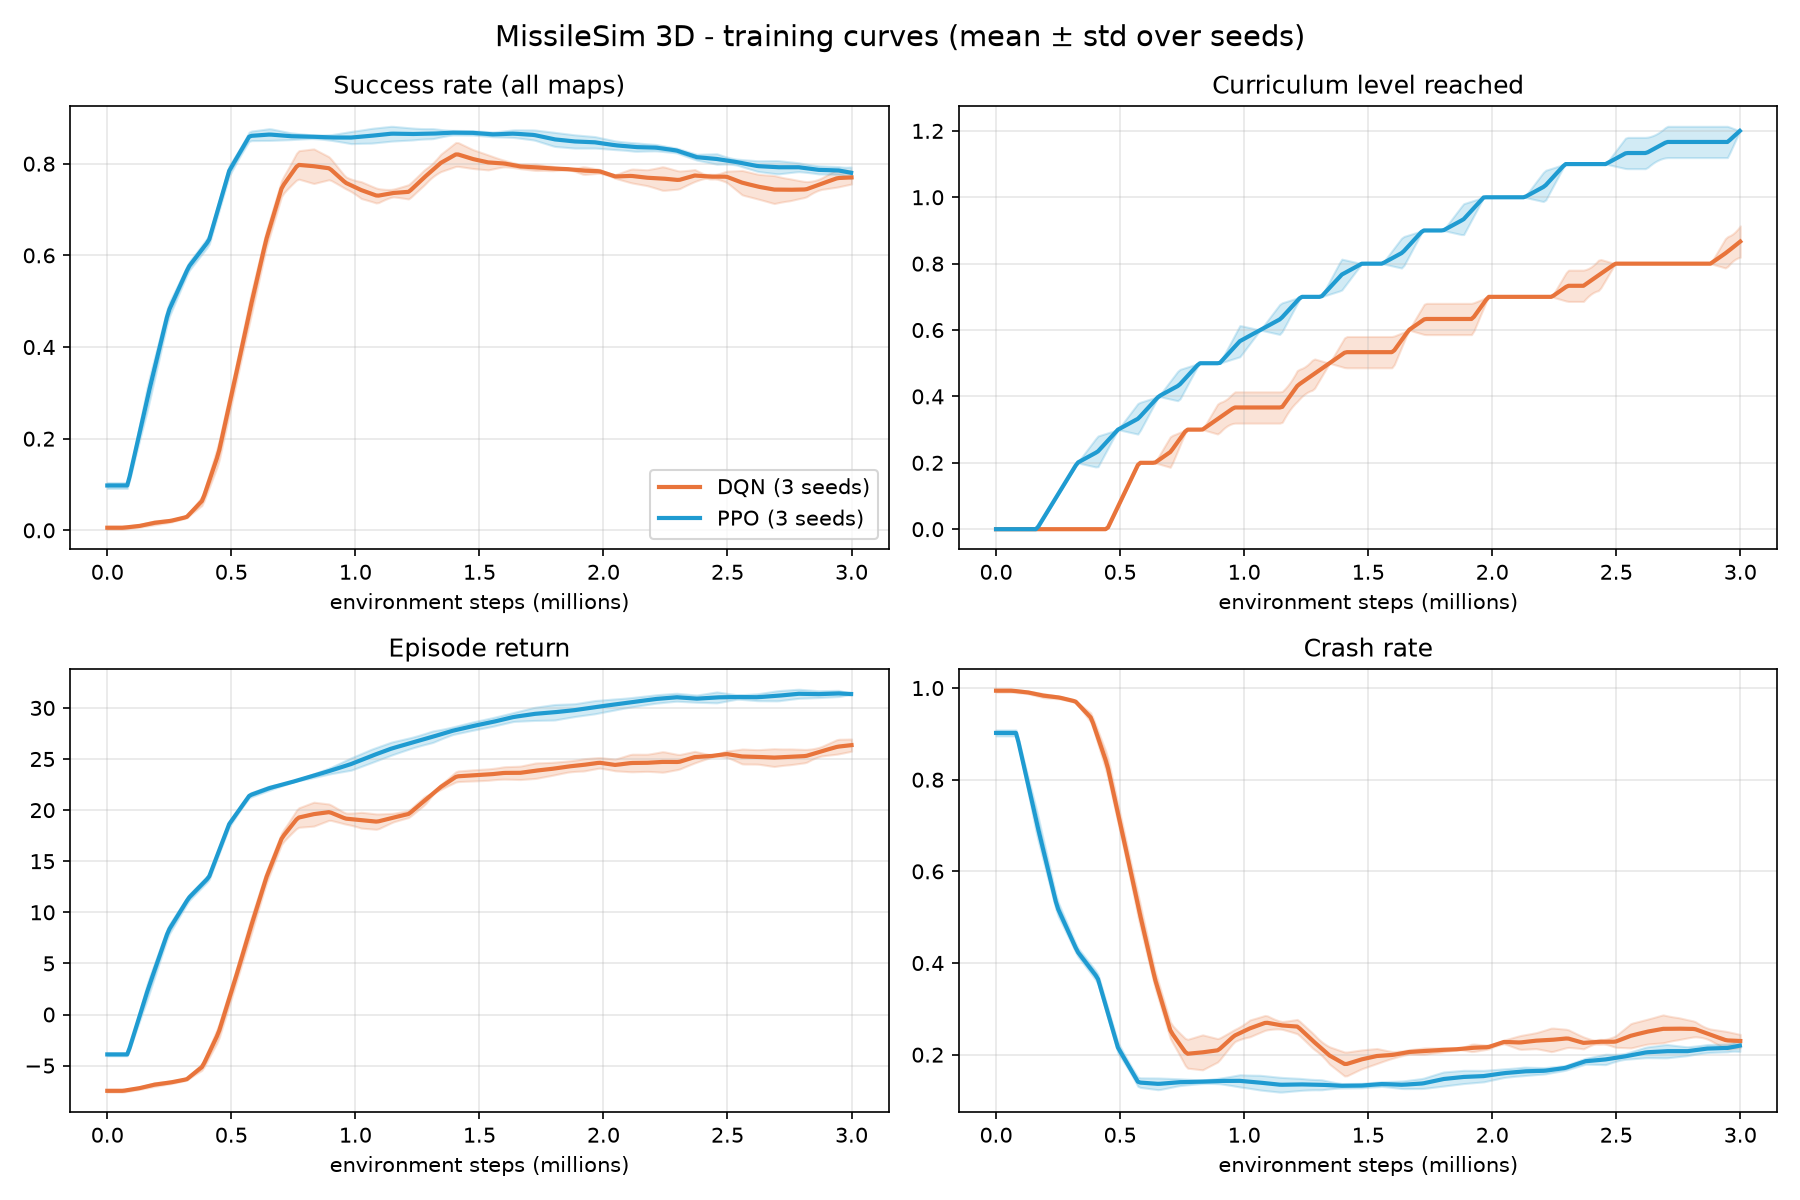
\includegraphics[width=0.78\textwidth]{training_curves.png}
\vspace{-4pt}
\caption{Training curves (mean $\pm$ std over 3 seeds). Success and crash rates are measured on the
maps of the current curriculum level, so they dip as the curriculum makes maps harder.}
\end{figure*}
\section{RL Formulation}
\textbf{State space} $\mathcal{S}\subset\mathbb{R}^{61}$ (continuous, normalised):
a $5{\times}5$ grid of ray-cast distances in a $70^\circ$ cone ahead of the nose (range 40, scaled
to $[0,1]$) at time $t$ \emph{and} $t{-}1$, so that obstacle motion is observable (50); the unit
vector to the target in the missile's body frame (3); distance to target (1); speed (1); pitch (1);
$\sin\psi,\cos\psi$ (2); position in the cross-section $y/8,z/8$ (2); remaining tunnel length (1).
\textbf{Action space} $\mathcal{A}$ (discrete, $|\mathcal{A}|{=}7$): coast, pitch up, pitch down,
yaw left, yaw right, boost, brake (i.e.\ $u_\theta,u_\psi,u_v\in\{-1,0,1\}$, one at a time).
\textbf{Reward.} With $d_t$ the distance to the target,
\begin{equation*}
r_t = 0.1\,(d_{t-1}-d_t) - 0.01 + 20\,\mathbb{1}_{\text{hit}} - 10\,\mathbb{1}_{\text{crash}}
      - 5\,\mathbb{1}_{\text{timeout}} .
\end{equation*}
The dense progress term guides learning, the step penalty discourages dawdling, and the terminal
terms encode the true objective. A \emph{hit} is $\|\mathbf{p}-\mathbf{p}_{\text{tgt}}\|<2.2$; a
\emph{crash} is contact with a wall, pipe or gate; a \emph{timeout} occurs after
$\lceil 1.8(L{+}6)/(8\Delta t)\rceil$ steps. Timeouts are treated as truncations (bootstrapped),
crashes and hits as true terminals.

\section{Algorithms and Baselines}
Both agents are implemented directly in PyTorch, without RL libraries.
\textbf{PPO}~\cite{schulman2017} (main): separate actor and critic MLPs ($2{\times}256$, ReLU,
orthogonal init.), clipped surrogate objective
$L=\mathbb{E}\big[\min(\rho_tA_t,\mathrm{clip}(\rho_t,0.8,1.2)A_t)\big]$ with
GAE~\cite{schulman2016} ($\gamma{=}0.995,\lambda{=}0.95$), entropy bonus 0.01, value loss 0.5,
rollouts of $32{\times}128$ steps, 4 epochs $\times$ 4 minibatches, Adam $3{\cdot}10^{-4}$ with
linear annealing, gradient clip 0.5.
\textbf{DQN}~\cite{mnih2015} (baseline): Double DQN~\cite{vanhasselt2016} with a dueling
head~\cite{wang2016}, 3-step returns, Huber loss, replay buffer $3{\cdot}10^{5}$, batch 256,
soft target update $\tau{=}0.005$, $\epsilon$: $1\to0.03$ over the first 20\% of training,
$\gamma{=}0.99$, Adam $3{\cdot}10^{-4}$.
\textbf{Baselines:} a uniform \emph{random} policy, and a hand-coded \emph{steer-to-target}
rule that turns toward the target and ignores obstacles (used only for comparison).
\textbf{Protocol.} Each algorithm: 3 seeds $\times$ $3{\cdot}10^{6}$ environment steps, with
identical curriculum (PPO $\approx$11 min, DQN $\approx$16 min per run on a desktop CPU).
Evaluation: greedy policy, 300 held-out maps per level (separate seed), identical maps for all
policies.

\section{Results}
\begin{table}[h]
\centering\small
\caption{Success rate (\%) on unseen maps, mean $\pm$ std over 3 seeds.}
\setlength{\tabcolsep}{2.6pt}
\begin{tabular}{lccccc}
\toprule
Policy & $\ell{=}0$ & 0.5 & 1.0 & 1.5 & 2.0\\
\midrule
Random & 1.0 & 0.0 & 0.0 & 0.0 & 0.0\\
Steer rule & 49.0 & 3.3 & 0.0 & 0.0 & 0.0\\
DQN & 95.1{\scriptsize$\pm$1.9} & 88.9{\scriptsize$\pm$2.6} & 47.0{\scriptsize$\pm$3.8} & 8.1{\scriptsize$\pm$2.7} & 0.4{\scriptsize$\pm$0.5}\\
PPO & \textbf{99.5}{\scriptsize$\pm$0.4} & \textbf{94.8}{\scriptsize$\pm$0.4} & \textbf{85.5}{\scriptsize$\pm$0.7} & \textbf{55.3}{\scriptsize$\pm$4.6} & \textbf{14.2}{\scriptsize$\pm$3.0}\\
\bottomrule
\end{tabular}
\end{table}
\begin{figure}[h]
\centering
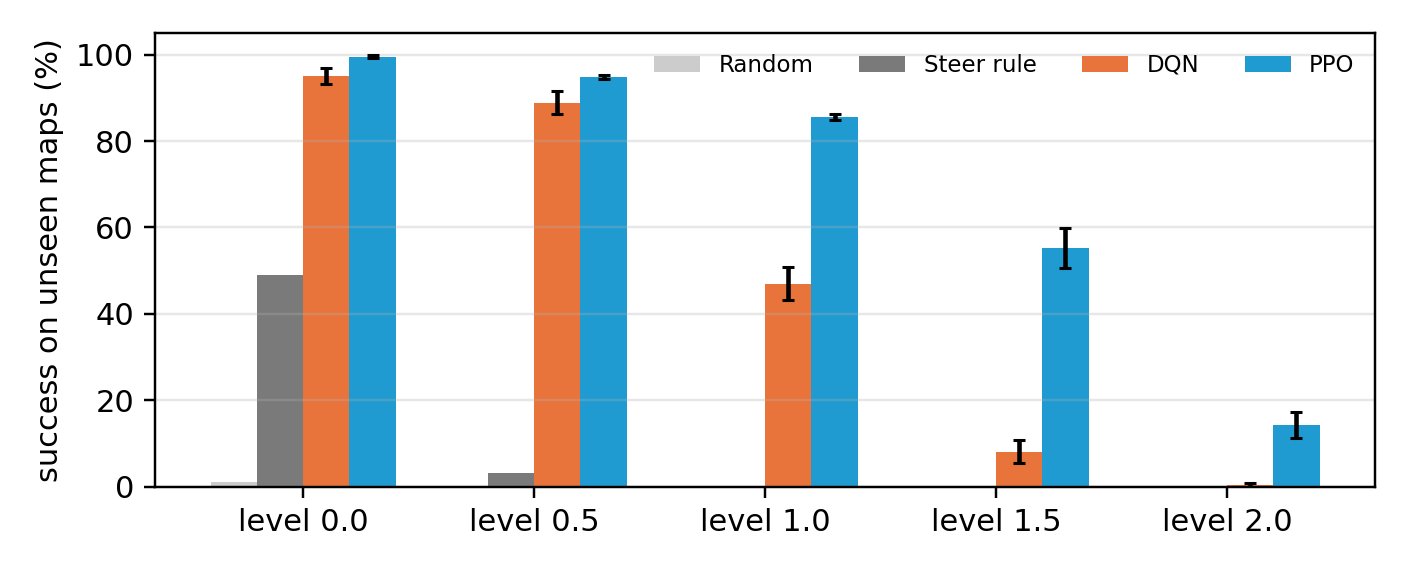
\includegraphics[width=\columnwidth]{eval_compact.png}
\caption{Held-out evaluation by difficulty level (error bars: std over seeds).}
\end{figure}

Both RL agents learn to avoid obstacles far beyond the steer-to-target rule, which succeeds on
49\% of the easiest maps but almost never once gates and moving pipes appear: obstacle
avoidance is essential and is learned, not hand-coded. PPO is better at every level and climbs the
curriculum faster (level 1.2 vs.\ 0.87 after $3{\cdot}10^{6}$ steps), and the gap widens with
difficulty (85.5\% vs.\ 47.0\% at $\ell{=}1$; 55.3\% vs.\ 8.1\% at $\ell{=}1.5$). PPO also
generalises into the expert tier beyond the level it trained on (14\% at $\ell{=}2$).
Seed-to-seed variance is small for both methods, so the conclusions are robust.

\begin{figure}[h]
\centering
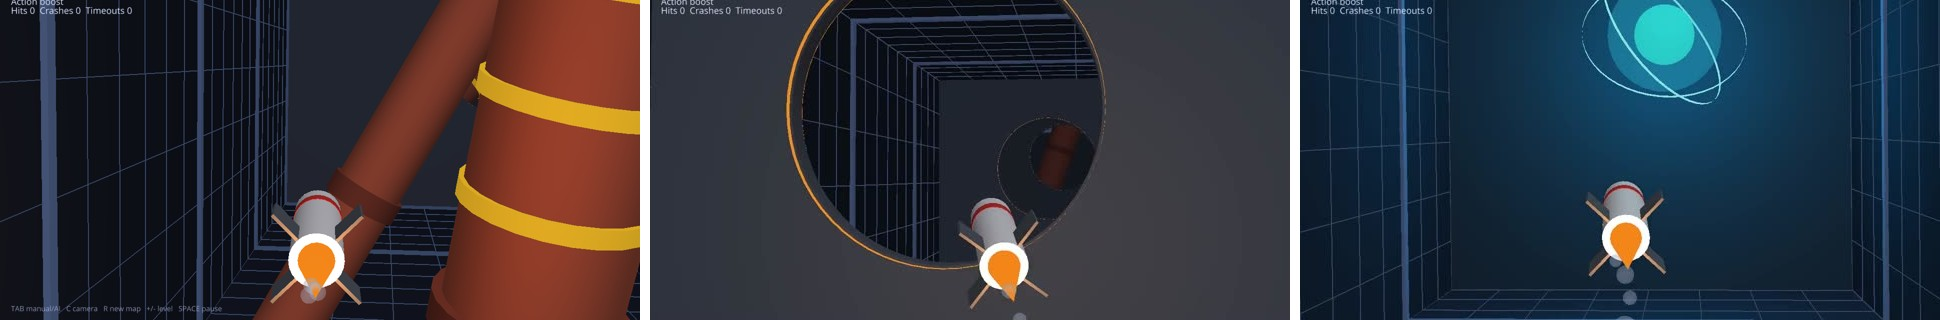
\includegraphics[width=\columnwidth]{scenes.jpg}
\caption{The trained PPO agent in the 3D viewer on unseen maps: dodging moving pipes (striped),
threading a gate hole, and approaching the target core.}
\end{figure}
\section{Discussion}
PPO's advantage grows with difficulty. Plausible explanations (not tested separately here) are its
stable on-policy updates over large batches from many parallel environments, and that DQN's replay
buffer keeps mixing in transitions from earlier, easier curriculum levels, so its value estimates lag
behind the changing map distribution.
\textbf{Limitations:} simplified arcade dynamics (no aerodynamics or roll), discrete actions, and a
fixed training budget; the expert tier remains unsolved, suggesting longer training, recurrent
policies or continuous control as future work.
A 3D viewer (Ursina) renders trained policies and supports human play for comparison.

\vspace{-6pt}
{\footnotesize
\begin{thebibliography}{9}\setlength{\itemsep}{0pt}
\bibitem{mnih2015} V.~Mnih et al., ``Human-level control through deep reinforcement learning,'' \emph{Nature}, 518, 2015.
\bibitem{schulman2017} J.~Schulman, F.~Wolski, P.~Dhariwal, A.~Radford, O.~Klimov, ``Proximal policy optimization algorithms,'' arXiv:1707.06347, 2017.
\bibitem{schulman2016} J.~Schulman, P.~Moritz, S.~Levine, M.~Jordan, P.~Abbeel, ``High-dimensional continuous control using generalized advantage estimation,'' \emph{ICLR}, 2016.
\bibitem{vanhasselt2016} H.~van Hasselt, A.~Guez, D.~Silver, ``Deep reinforcement learning with double Q-learning,'' \emph{AAAI}, 2016.
\bibitem{wang2016} Z.~Wang et al., ``Dueling network architectures for deep reinforcement learning,'' \emph{ICML}, 2016.
\bibitem{bengio2009} Y.~Bengio, J.~Louradour, R.~Collobert, J.~Weston, ``Curriculum learning,'' \emph{ICML}, 2009.
\bibitem{cobbe2019} K.~Cobbe, O.~Klimov, C.~Hesse, T.~Kim, J.~Schulman, ``Quantifying generalization in reinforcement learning,'' \emph{ICML}, 2019.
\end{thebibliography}}
\end{document}
